\documentclass{beamer}
\usepackage[english]{babel}
\usepackage[utf8]{inputenc}
\usepackage[T1]{fontenc}
\usepackage{lmodern}
\usepackage{hus-beamer} 
\usepackage{ifthen}
\usepackage[bibstyle=authoryear, citestyle=authoryear, maxcitenames=2, maxbibnames=2, backend=bibtex]{biblatex}
%\usepackage[maxbibnames=2]{biblatex}
%citestyle=authoryear or numeric or ...
\addbibresource{ref.bib}

%------ tikZ ------%
\usepackage{tikz}
\usetikzlibrary{positioning, arrows}
\usetikzlibrary{backgrounds}

\mode<presentation>{
	\usefonttheme{professionalfonts} % normal font for math formulas
	% insert section page with title only
	% before each section
	\AtBeginSection[]{
	\begin{frame}%[noframenumbering] % remove this if you do not want to number section page
	\vfill
	\centering
	\begin{beamercolorbox}[sep=8pt,center,shadow=true,rounded=true]{title}
	\usebeamerfont{title}\insertsectionhead\par%
	\end{beamercolorbox}
	\vfill
	\end{frame}
}
}
%%%%%%%%
%\AtBeginBibliography{\footnotesize} % Footnotesize for Bibliography entries

% \setbeamertemplate{bibliography item}{%
%   \ifboolexpr{ test {\ifentrytype{book}} or test {\ifentrytype{mvbook}}
%     or test {\ifentrytype{collection}} or test {\ifentrytype{mvcollection}}
%     or test {\ifentrytype{reference}} or test {\ifentrytype{mvreference}} }
%     {\setbeamertemplate{bibliography item}[book]}
%     {\ifentrytype{online}
%        {\setbeamertemplate{bibliography item}[online]}
%        {\setbeamertemplate{bibliography item}[article]}}%
%   \usebeamertemplate{bibliography item}}

% \defbibenvironment{bibliography}
%   {\list{}
%      {\settowidth{\labelwidth}{\usebeamertemplate{bibliography item}}%
%       \setlength{\leftmargin}{\labelwidth}%
%       \setlength{\labelsep}{\biblabelsep}%
%       \addtolength{\leftmargin}{\labelsep}%
%       \setlength{\itemsep}{\bibitemsep}%
%       \setlength{\parsep}{\bibparsep}}}
%   {\endlist}
%   {\item}


%\defbibheading{bibliography}[\refname]{}

%------------------%

\begin{document}
\title{Improving Performance}
\subtitle{Week 4}
\author{COMP6252 (Deep Learning Technologies)}
\institute[ECS, University of Southampton]{ECS, University of Southampton} \date{28 April 2022}

\begin{frame}[plain,noframenumbering]
    \placelogofalse % No logo at the title page
    \titlepage
\end{frame}
    
\placelogotrue

    
\renewcommand{\figurename}{From}
\begin{frame}
    \frametitle{Introduction}
\begin{itemize}
    \item As we have already  seen DNN are powerful models.
    \item This is mainly due to their strong expressiveness: 
    \begin{itemize}
        \item  the ability to model complicated relationships between input and output
    \end{itemize}
   
    \item But this same expressiveness can lead to some problems
\end{itemize}
    \begin{enumerate}
        \item Overfitting
        \begin{itemize}
            \item Due to their power, NN can "learn" noise present in the training but not in the test datasets 
            \item This reduces their generalization efficacy
        \end{itemize}
        \item Convergence 
        \begin{itemize}
            \item Training takes long time. Sometimes doesn't even converge
            \item The results highly dependent on the meta parameters 
        \end{itemize}
    \end{enumerate}

\end{frame}
\begin{frame}
    \frametitle{What can be done?}
    This week we will introduce three approaches to mitigate the problems of convergence and overfitting.

    \begin{enumerate}
        \item Early stopping
        \item Dropout
        \item Batch normalization 
    \end{enumerate}
\end{frame}

\begin{frame}
    \frametitle{Overfitting}
\begin{itemize}
    \item An example of overfitting is shown below 
    \item The training accuracy keeps increasing while the validation plateau and even decreases
\end{itemize}
\begin{center}
    \begin{figure}
     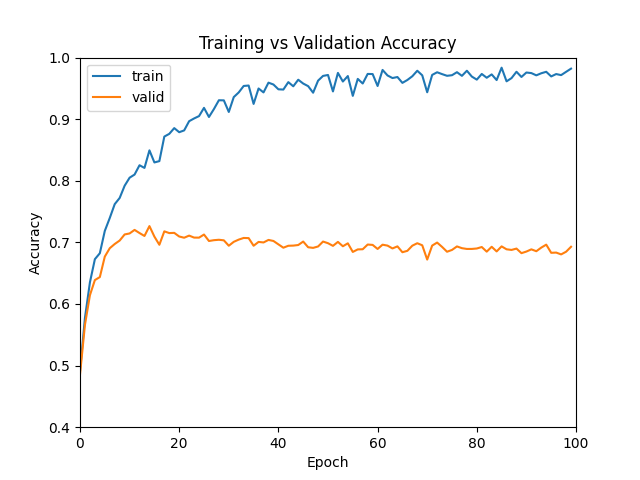
\includegraphics[width=0.7\textwidth]{figs/train-vs-valid-acc.png}
        
    \end{figure}
\end{center}

\end{frame}


\begin{frame}
    \frametitle{Early stopping}
    \begin{itemize}
        \item In the previous figure, the max accuracy occurs at epoch 14
        \item If we stop training at epoch 14 or close to it not only we get better accuracy but we save lots of time 
        \item This is exactly what is called \textbf{early stopping}
        \item How do we know when to stop training?
        \item One of the simplest methods is to monitor the \textbf{validation loss}
    \end{itemize}
    

\end{frame}
\begin{frame}
    \frametitle{Validation loss vs accuracy}
\begin{itemize}
    \item Below is a plot of validation accuracy vs loss.
    \item Loss was multiplied by 0.5 to show them both on the same plot
    \item It is clear that accuracy plateaus after the loss starts increasing
\end{itemize}
\begin{center}
    \begin{figure}
     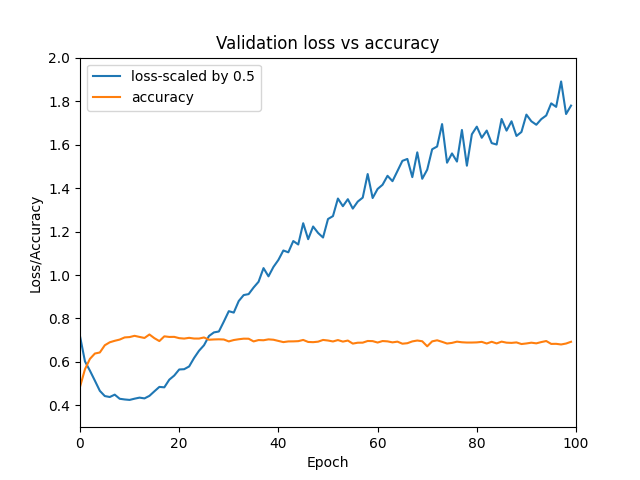
\includegraphics[width=0.7\textwidth]{figs/valid-loss-vs-accuracy1.png}
        
    \end{figure}
\end{center}

\end{frame}\begin{frame}
    \frametitle{A zoomed view}
    \begin{itemize}
        \item Below is a zoomed view of the previous figure
        \item A vertical line passing by epoch 14 (where max accuracy occurs) is shown 
    \end{itemize}
    \begin{figure}
        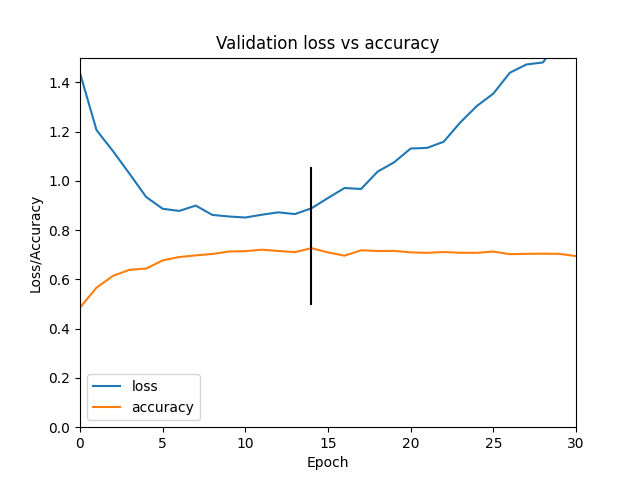
\includegraphics[width=0.7\textwidth]{figs/valid-loss-vs-accuracy.png}
           
       \end{figure}
    

\end{frame}
\begin{frame}
    \frametitle{Dropout}
    \begin{itemize}
        \item Dropout is another method used to minimize overfitting 
        \item A dropout layer "drops" certain nodes from the NN as shown in the figure below
    \end{itemize}
    \begin{center}
        \begin{figure}
         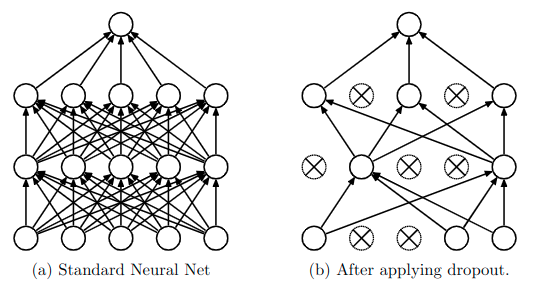
\includegraphics[width=0.7\textwidth]{figs/dropout.png}
            \caption{Srivastava et al.}
        \end{figure}
    \end{center}
    
\end{frame}
\begin{frame}
    \frametitle{What is happening exactly?}
    \begin{itemize}
        \item Every training pass \textbf{different} nodes are dropped 
        \item A neural network with $n$ nodes that uses dropout, can be seen as a set of $2^n$ different "smaller" networks. Why?
        \item It means that using dropout is equivalent to averaging over an ensemble of Neural networks sharing the same weights
        \item Since the noise learned by each "smaller" network is random, "averaging" makes them cancel each other.
    \end{itemize}

\end{frame}
\begin{frame}
    \frametitle{Implementation}
\begin{itemize}
    \item Using layers with an on/off switch on nodes is not practical 
    \item More importantly, with an NN with large number of nodes it is \textbf{impossible}
    \item Instead, a node is turned off by multiplying its output with zero \textbf{with probability} $p$ 
    \item Mathematically, let $\mathbf{y}^{l}$ be the output of layer $l$ in a fully connected network
    \item Then the output of layer $(l+1)$ is given by  (* is element wise product)
\end{itemize}
    \begin{align*}
       \mathbf{r}^l&=Bernoulli(p)\\
        \mathbf{\tilde{y}}^l&=\mathbf{r}^l*\mathbf{y}^l\\
        \mathbf{z}^{l+1}&=\mathbf{W}^{l+1}\mathbf{y}^l+\mathbf{b}^{l+1}\\
        \mathbf{y}^{l+1}&=\sigma(\mathbf{z}^{l+1})
    \end{align*}

\end{frame}
\begin{frame}
    \frametitle{What about testing?}
    \begin{itemize}
        \item We have seen that training a NN with dropout is   is equivalent to training multiple "smaller" networks.
        \item The result is an average over all such networks.
        \item To be consistent we must use the weights learned in the training phase for testing
        \item This means we have to \textbf{average} over all possible networks, which is infeasible.
        \item We approximate this averaging by \textbf{not using dropout} during testing
        \item But the weights obtained in the training phase are multiplied by the probability $p$
        \item Equivalently the weights are multiplied by $\frac{1}{p}$ during training
    \end{itemize}
    

\end{frame}

\begin{frame}
    \frametitle{Batch Normalization}
\begin{itemize}
    \item A Batch normalization layer transforms the distribution of the input to a distribution that has 0 mean and unit variance
    \item Batch normalization is a powerful method that 
    \begin{enumerate}
        \item Allows for better convergence of NN training 
        \item Adding BN layers to existing NN yield better generalization results
        \item Reduces over fitting
        \item Training is less sensitive to meta-parameters (learning rate, weights initialization)
    \end{enumerate}
    
\end{itemize}
    

\end{frame}
\begin{frame}
    \frametitle{Batch Normalization- How does it work}
    \begin{itemize}
        \item Given a mini-batch of tensors $x_{ci}$ of dimension (S,C,H,W)
        \item  where $c$ is the channel index and $i$ collectively refers to all other dimensions. 
        \item  Let $N=S\times H\times W$.
        \item Batch normalization computes the mean and variance of the batch (per channel) according to
    \end{itemize}
        \begin{align*}
        \mu_c&=\frac{1}{N}\sum_{i=1}^N x_{ci}\\
        \sigma^2_c&=\frac{1}{N}\sum_{i=1}^N \left(x_{ci}-\mu_c\right)^2
        \end{align*}
\end{frame}

\begin{frame}
    \frametitle{Batch Normalization- How does it work}
    The normalized inputs are computed as follows:
    
    \begin{align*}
    \hat{x}_{ci}=\frac{x_{ic}-\mu_c}{\sqrt{\sigma^2_c+\epsilon}}
    \end{align*}
Therefore, for each channel, the $\hat{x}_{ci}$ have zero mean and unit variance. The output of the batch normalization layer is given by
    
    \begin{align*}
    y_{ic}=\gamma \hat{x}_{ic}+\beta
    \end{align*}
    
    Where $\gamma$ and $\beta$ are \textbf{learnable} parameters.
\end{frame}

\begin{frame}
    \frametitle{Batch normalization - Why does it work?}
\begin{itemize}
    \item Considerable ongoing debate
\item In the original paper of \href{https://arxiv.org/abs/1502.03167}{\beamergotobutton{Ioffe and Szegedy }} it claims that it fixes the internal covariate shift 
\item meaning the change in the distribution due to the change of the weights during learning 
\item \href{https://arxiv.org/abs/1805.10694v1}{\beamergotobutton{Kohler et al.}} propose that it separates the change in magnitude from the change of directions.
\item This can be seen from the fact that the $\hat{x}_{ci}$ are normalized and all of them share the same magnitude $\gamma$

\end{itemize}
\end{frame}


\begin{frame}
    \frametitle{Example}
Consider a mini-batch of size two, containing the tensors of size $2\times 2$, $A$ and $B$ with both having a single channel.


\begin{columns}
    
    \begin{column}{0.5\textwidth}
        \[
    A=\begin{bmatrix}
        1 &2 \\
        3 & 4
    \end{bmatrix}    
    \]
    \end{column}
  \begin{column}{0.5\textwidth}
      \[
        B=\begin{bmatrix}
         5 &6 \\
         7 & 8
        \end{bmatrix}    
      \]
  \end{column}

\end{columns}
\begin{itemize}
    \item The mean is 4.5 and (biased) variance is 5.25 therefore the output is
\end{itemize}
 
\begin{columns}
    
    \begin{column}{0.45\textwidth}
        \[
    A=\left[\begin{smallmatrix}
        (1-4.5)/5.25 &(2-4.5)/5.25 \\
        (3-4.5)/5.25 & (4-4.5)/5.25
    \end{smallmatrix}    \right]
    \]
    \end{column}
  \begin{column}{0.45\textwidth}
    \[ 
        B=\left[\begin{smallmatrix}
         (5-4.5)/5.25 & (6-4.5)/5.25 \\
         (7-4.5)/5.25 & (8-4.5)/5.25
        \end{smallmatrix}\right]    
      \]
     
  \end{column}
  
\end{columns}
\begin{itemize}
    \item When the input has multiple channels, the same operation is performed for each channel independently
    \end{itemize}
\end{frame}



\begin{frame}
    \frametitle{In practice}
    \begin{itemize}
        \item Data: CIFAR10
        \item The NN has two convolutional blocks 
        \item The first contains two sub-blocks each with 
        \begin{enumerate}
            \item 32 filters with receptive field of 3x3 
            \item followed by BN layer
            \item followed by ReLU
        \end{enumerate}
        \item the sub-blocks are followed by a max pooling layer of size 2x2
       
        \item The second block is the same as the first but with 64 filter 
        \item The conv blocks are followed by two feedforward layers with 128 and 10 nodes respectively
    \end{itemize}
\end{frame}

\begin{frame}
    \frametitle{Nework Architecture}

    \begin{center}
        
        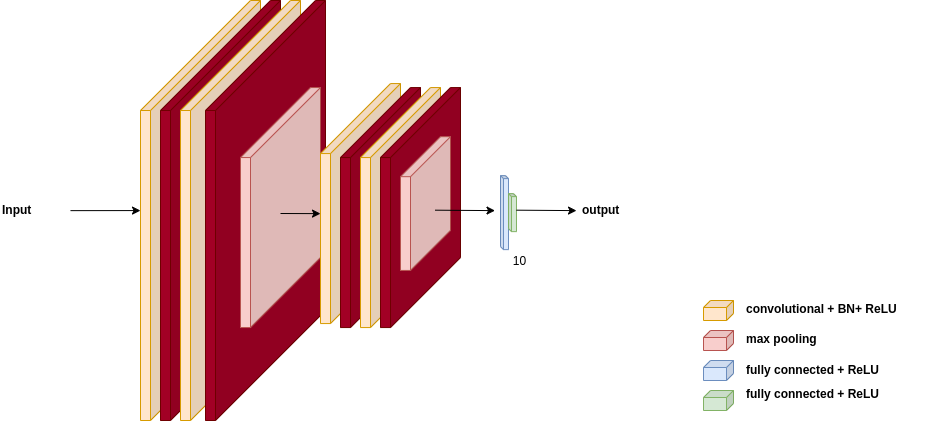
\includegraphics[width=1.1\textwidth]{figs/conv-with-bn.png}
    \end{center}
\end{frame}


\begin{frame}
    \frametitle{Results: validation accuracy of BN vs no BN}
    \begin{center}
        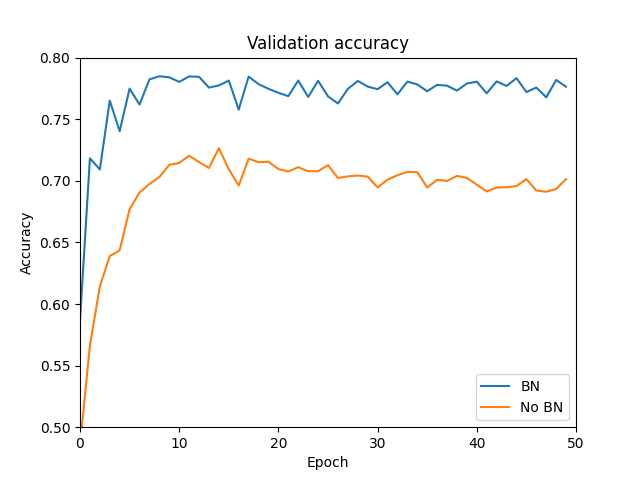
\includegraphics[width=0.9\textwidth]{figs/accuracy-BN-vs-NoBN.png}
    \end{center}
\end{frame}

\begin{frame}
    \frametitle{Results: train-vs-validation accuracy with BN}
    \begin{center}
        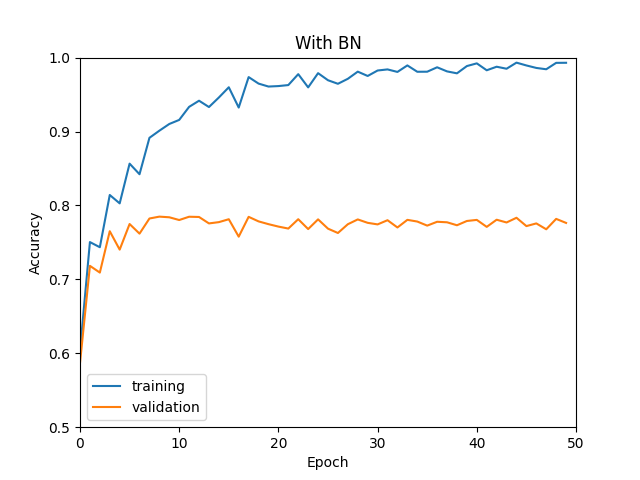
\includegraphics[width=0.9\textwidth]{figs/accuracy-t-vs-v-BN.png}
    \end{center}
\end{frame}


\begin{frame}
    \frametitle{Analysis of results}
\begin{itemize}
    \item Batch normalization give much better accuracy.
    \item Peak value for the accuracy  for BN is 78\% vs  72\%
    \item The average after the peak for BN is vs 75\% vs 69\%
    \item Also, with BN the peak acc is reached after 8 epochs vs 14 without BN.
\end{itemize}
    \end{frame}


\begin{frame}
    \frametitle{Results: train-vs-validation accuracy without BN}
    \begin{center}
        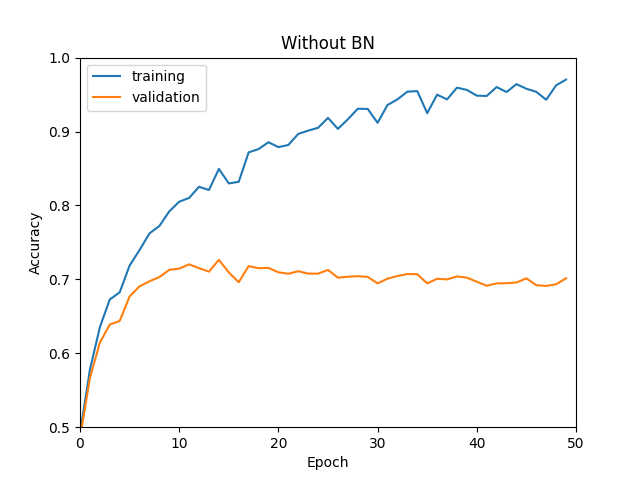
\includegraphics[width=0.9\textwidth]{figs/accuracy-t-vs-v-woBN.png}
    \end{center}
\end{frame}

\begin{frame}
    \frametitle{References}
    % \begin{itemize}
    %     \item \cite{srivastava14}\cite{ioffe15}
    % \end{itemize}
\nocite{*}    
\printbibliography
\end{frame}

\end{document}